\documentclass{article}

\usepackage{inputenc}[utf8]
\usepackage[T1]{fontenc}
\usepackage[a4paper]{geometry}
\usepackage{fancyhdr}
\usepackage{url}
\usepackage{hyperref}
\usepackage[ngerman]{babel}
\usepackage{graphicx}
\usepackage{pgfplots}
\usepackage{amsmath}
\usepackage{amssymb}

% Generate external pdf and import
\pgfplotsset{width=9cm,compat=1.9}

\title{{\Huge Aufgabenblatt 03}\\Einführung in die Kryptographie PS}
\author{Andreas Schlager}


\begin{document}
    \pagestyle{fancy}
    \fancyhead{}
    \fancyhead[L]{Aufgabenblatt 03}
    \fancyhead[R]{Einführung in die Kryptographie}
    \fancyfoot{}
    \fancyfoot[L]{Andreas Schlager}
    \fancyfoot[R]{\thepage}
    \maketitle
    \tableofcontents
    \section{Aufgabe 10}
    \textit{Fortsetzung Aufgabe 9.) Simulieren sie verschiedene Arten von biometrischer Varianz, 
    die sich als gleichverteilte Bitfehler steigender Anzahl oder Bursts (gehäufte
    Fehler an einer oder mehreren Stellen) manifestieren. Wenden sie verschiedene
    Hamming-Codes zur Fehlerkorrektur an. Dokumentieren sie die Auswirkung von
    verschiedenen Fehlerarten (Quantität, Qualität) auf die Möglichkeit, den Schlüssel
    tatsächlich korrekt zu erzeugen.}\vspace*{1em}\newline
    Ein regulärer Hamming-Code ist in der Lage 1-Bit-Fehler zu korrigieren und 2-Bit-Fehler zu erkennen.
    Würde man die Länge des Codes genau an den Schlüssel $S$ oder die biometrischen Daten $X$ anpassen,
    könnte man demnach auch nur einen Bit-Fehler durch die Messung korrigieren. In den meisten Fällen variiert die Messung
    jedoch stärker als nur ein einzelnes verändertes Bit. Die Lösung ist den Schlüssel in mehrere Blöcke
    entsprechender Größen aufzuteilen und anschließend aus jedem einen Hamming Code zu generieren. Treten 
    nun Fehler in unterschiedlichen Blöcken auf, können diese ohne Probleme korrigiert werden, wobei
    zwei oder mehr Fehler im gleichen Block nach wie vor nicht behoben werden können. In wie viele Blöcke man 
    den Schlüssel segmentieren sollte, hängt davon ab welchen Grad der Fehlerkorrektur und wie viel Redundanz
    man möchte. Kleine Blöcke, also kürzere Hamming Codes, führen zu einer größeren Redundanz 
    (siehe Abbildung \ref{fig:redundancyvsdata}.) und somit zu einer verbesserten Messtoleranz, 
    die benötigte Datenmenge steigt jedoch ebenfalls.
    
    \begin{figure}
    \centering
    \begin{tikzpicture}
        \begin{axis}[
            xbar stacked,
            bar width=15pt,
            nodes near coords,
            enlargelimits=0.15,
            legend style={at={(0.5,-0.20)},
              anchor=north,legend columns=-1},
            xlabel={data redundancy ratio},
            symbolic y coords={H{(128,120)}, H{(64,57)}, H{(32,26)}, H{(16,11)}, H{(8,4)}},
            ytick=data,
            xmin=0,xmax=100,
            xticklabel={\pgfmathprintnumber{\tick}\%}
            ]
        \addplot+[xbar] plot coordinates {(93.75,H{(128,120)}) (89,H{(64,57)}) (81.25,H{(32,26)}) (68.75,H{(16,11)}) (50,H{(8,4)})};
        \addplot+[xbar] plot coordinates {(6.25,H{(128,120)}) (11,H{(64,57)}) (18.75,H{(32,26)}) (31.25,H{(16,11)}) (50,H{(8,4)})};
        \legend{\strut data, \strut parity}
        \end{axis}
    \end{tikzpicture}
    \label{fig:redundancyvsdata}
    \caption{Daten vs. Redundanz der unterschiedlichen Hamming-Codes}
\end{figure}

    Um diesen Trade-off zu visualisieren, werden unterschiedliche Hamming-Code-Größen verglichen, wobei verschiedene
    Arten von Bitfehlern (gleichverteilt, oder burst) auftreten. Hierbei ist $H(n, d)$ ein $n$-Bit langer Hamming-Code
    mit $d$ Datenbits und $n-d$ Paritätsbits.
    In der Simulation werden folgende Hamming-Code Blockgrößen getestet:
    \[
        \begin{array}{ccccc}
            H(8,4) & H(16,11) & H(32,26) & H(64,57) & H(128,120)
        \end{array}
    \]
    \subsection{Code}
    Der Funktionsweise des Code aus Aufgabe 9.) ist im wesentlichen gleich geblieben, wobei die Hamming-Code Bibliothek um die 
    Funktionalität der Segmentierung in die gewünschten Blockgrößen erweitert wurde. So führt ein Aufruf
    der Funktion \verb|hamming::encode(data, n)| dazu, dass die Daten in entsprechenden viele $H(n,d)$ Codes
    aufgeteilt werden. Angenommen es werden $x$-Bits in $H(n,d)$ Blöcke überführt, gäbe es pro Block $d$ Datenbits.
    Die Anzahl der dadurch entstehenden Blöcke entspricht
    \begin{equation} \label{eq:1}
        \#\text{Blöcke}=\left\lceil\frac{x}{d}\right\rceil.
    \end{equation}
    \begin{figure}[h]
        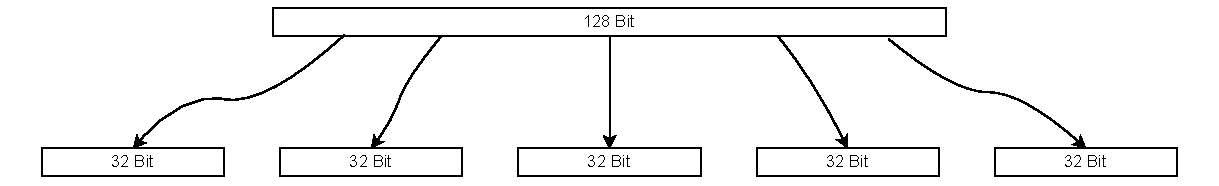
\includegraphics[width=\textwidth]{img/segmentation.pdf}
        \caption{Segmentierung von 128-Bits auf fünf $H(32,26)$ Codes}
        \label{fig:segmentation}
    \end{figure}
    Füllen die Daten die Hamming Blöcke nicht vollständig aus, werden sie mit Nullen ergänzt. Teilt man also einen
    128-Bit Datenblock auf fünf $H(32,26)$ Codes auf, wären im letzten Block noch 24-Datenbits und zwei Füllbits.
    Für das FCS wird wieder ein zufälliger 128-Bit Schlüssel $S$ erstellt, welcher dann in mehrere Hamming-Code-Blöcke kodiert wird.
    Die Blockgrößer wird über \verb|hamming_block_size| bestimmt und nimmt in der Simulation die Werte $\left[8,16,32,64,128\right]$
    an. Die Blöcke werden anschließend in einen durchgängigen Block umgewandelt, um die Kombination mit der biometrischen Probe
    zu vereinfachen.
    \begin{verbatim}
fn fcs_run(hamming_block_size: usize, flip_amount: usize) -> bool {
    let s = rng().random_iter().take(16).collect::<Vec<u8>>();
    let hs = hash(&s);
    let c = hamming::encode(&s, hamming_block_size)
        .expect("encode failed")
        .to_continuous();
    // ...
}
    \end{verbatim}
    Als nächstes wird eine biometrische Probe $X$ zufällig generiert, wobei die Probe gleich groß wie der Schlüssel $S$ ist.
    Um $X$ und $C$ zu kombinieren, müssen beide gleich groß sein. Durch die Paritäts- und Füllbits ist allerdings $|C|>|X|$.
    Um dieses Problem zu umgehen wird $X$ ebenfalls Hamming-kodiert und dadurch ebenfalls durch Füllbits ergänzt.
    \begin{verbatim}
let x = rng().random_iter().take(s.len()).collect::<Vec<u8>>();
let x = hamming::encode(&x, hamming_block_size)
    .expect("encode failed")
    .to_continuous();

let w = fuse(&c, &x);
    \end{verbatim}
    Die Messvariation wird simuliert, indem zufällige Bits von $X$ gekippt werden. Für diesen Zweck gibt es zwei unterschiedliche
    Funktionen: \verb|random_bit_flip| und \verb|burst_error|.
    \begin{verbatim}
let y = random_bit_flip(&x, flip_amount);
// oder
let y = burst_error(&x, rng().random_range(0..s.len()*8), flip_amount);
    \end{verbatim}
    Anschließend wird $Y$ mit $W$ kombiniert um das Codewort $C'$ zu erhalten, welches fehlerkorrigiert wird. Zu diesem Zeitpunkt
    besteht $C'$ noch immer aus den einzelnen Hamming-Blöcken. Um den Schlüssel $S'$ zu erhalten, müssen die Datenbits aus dem
    Code extrahiert werden.
    \begin{verbatim}
let c_prime = fuse(&w, &y);

let mut ecc = HammingCode::from_continuous(c_prime, hamming_block_size);
ecc.error_correct();

let s_prime = ecc.extract(s.len() * 8);
    \end{verbatim}
    Zuletzt werden die Hashwerte verglichen, um festzustellen, ob der Authentifizierung erfolgreich war.
    \begin{verbatim}
let hs_prime = hash(&s_prime);
hs == hs_prime
    \end{verbatim}
    \subsubsection{Simulation}
    Für die Simulation werden 1-15 Bitfehler (in gleichverteilt und burst Variante) mit den unterschiedlichen
    Hamming Codes jeweils 50 Mal getestet. Die Anzahl der erfolgreichen Authentifizierungsversuche wird gezählt und auf
    der Konsole ausgegeben.
    \begin{verbatim}
for flip_amount in 1..=15 {
    print!("{flip_amount}\t");
    for block_size in [8, 16, 32, 64, 128] {
        let successful_attempts = (0..50)
            .map(|_| fcs_run(block_size, flip_amount))
            .filter(|&r| r)
            .count();
        print!("{successful_attempts}\t");
    }
    println!();
}
    \end{verbatim}
    \subsection{Ergebnisse}
    Im Allgemeinen ergab die Simulation, dass die Toleranz der Messung durch die Segmentierung in kleinere Codes
    steigt. Das war zu erwarten, da die Redundanz bei kleineren Codes größer ist und somit mehr Bits für die
    Fehlerkorrektur verfügbar sind. Die Simulation ergab außerdem, dass Burstfehler für Hamming Codes Schwierigkeiten
    bereiten, da häufiger mehrere Fehler in den gleichen Blöcken auftreten.
    \subsubsection{Gleichverteilte Bitfehler}
    Bei den Ergebnissen (siehe Tab. \ref{tab:uniform_result}.) ist klar zu erkennen, dass durch die Segmentierung 
    mehrere zufällig Fehler erkannt und korrigiert werden konnten.
    Nicht besonders überraschend ist auch, dass 1-Bit Fehler von jedem Code in allen 50 Versuchen korrigiert 
    wurden. Der $H(8,4)$-Code war in der Lage im Durchschnitt die meisten Bitfehler zu korrigieren, da die
    Hälfte des Codes Redundanz ist. Außerdem ist erkenntlich: Je länger der Code (also weniger Redundanz), desto
    weniger Bits können korrigiert werden. Eine Überraschung war, dass der $H(128,120)$-Code es manchmal schaffte
    einen großen Bitfehler zu korrigieren. Um zu verstehen wieso es trotz des großen Fehlers zu einer erfolgreichen
    Authentifizierung kam, muss man sich überlegen wie der Schlüssel in den Blöcken positioniert ist.\newline
    Der Schlüssel wurde aus 128 zufälligen Bits konstruiert und in einen $H(128,120)$-Code umgewandelt.
    Wegen der Gleichung \ref{eq:1} ergeben sich zwei 128-Bit Blöcke, mit Platz für jeweils 120-Datenbits.
    Der Schlüssel füllt nun die 120-Bit des ersten Blocks vollständig aus und die übrigen acht Bit kommen
    in den zweiten Block. Das bedeutet, der zweite Block beinhaltet acht Schlüsselbits und \textbf{112 Füllbits}.
    Um die Berechnung zu vereinfachen wird näherungsweise angenommen, dass der zweite Block ausschließlich aus
    Füllbits besteht. Sei $X$ eine Zufallsvariable, die den Block beschreibt, in dem ein zufälliges Bit 
    gekippt ist. Da beide Blöcke gleich groß sind und die Wahrscheinlichkeit der Position des gekippten Bits
    gleichverteilt ist, folgt für die Wahrscheinlichkeiten $P(X=x)$
    \[
        P(X=1) = P(X=2) = 0.5.
    \]
    Sei außerdem $Y$ eine Zufallsvariable, welche die Anzahl der gekippten Bits im ersten Block beschreibt.
    Betrachtet man beispielsweise den Fall von 6-Bitfehlern, dann ist für eine erfolgereiche Authentifizierung
    höchsten ein Fehler im ersten Block erlaubt.
    \begin{align*}
        P(Y \leq 1) &= P(Y = 0) + P(Y = 1) = P(X=2)^{6} + {6\choose 1}P(X=1)^1P(X=2)^{5}\\
        &=0.5^{6} + 6\cdot 0.5^1 \cdot 0.5^5 = 0.109375
    \end{align*}
    \[
        \mathbb{E}\left[\text{"'erfolgreiche Authentifizierungen"'}\right] =  50 \cdot 0.109375 = 5.46875
    \]
    Im Schnitt erwartet man also bei dieser Implementierung des FCS und sechs gleichverteilten Bitfehlern 
    ungefähr $5.47$ erfolgereiche Authentifizierungen. Diese Tatsache spiegelt sich auch in der Ergebnistabelle 
    \ref{tab:uniform_result} wieder.

    \begin{table}[h!]
    \centering
    \begin{tabular}{c|ccccc}
        \#Errors & H(8,4) & H(16,11) & H(32,26) & H(64,57) & H(128,120)\\\hline
        1 &      50 &      50&      50&      50&      50\\      
        2 &      49 &      46&      35&      36&      39\\      
        3 &      46 &      42&      20&      22&      20\\      
        4 &      43 &      35&      11&      5&       7 \\      
        5 &      37 &      24&      6 &      1&       9 \\      
        6 &      29 &      11&      2 &      1&       5 \\      
        7 &      30 &      6 &      0 &      0&       1 \\      
        8 &      26 &      6 &      0 &      1&       0 \\      
        9 &      24 &      3 &      0 &      0&       2 \\      
        10&      19 &      1 &      0 &      0&       1 \\      
        11&      11 &      2 &      0 &      0&       0 \\      
        12&      9  &      0 &      0 &      0&       0 \\      
        13&      10 &      0 &      0 &      0&       0 \\      
        14&      6  &      0 &      0 &      0&       0 \\      
        15&      6  &      0 &      0 &      0&       0
    \end{tabular}
    \caption{Erfolgreiche Authentifizierungsversuche (Code vs. Anzahl der gleichverteilten Bitfehler)}
    \label{tab:uniform_result}
\end{table}
    \subsubsection{Burstfehler}  
    Die Simulation-Ergebnisse (siehe Tabelle \ref{tab:burst_result}.) zeigen, dass Burstfehler eine besondere Herausforderung für die Hamming-Codes darstellen. 
    Da sich die Fehler über mehrere aufeinanderfolgende Bits erstrecken, kommt es häufiger vor, dass mehrere Fehler 
    innerhalb desselben Blocks auftreten. Besonders bei längeren Codes mit geringerer Redundanz führte dies dazu, 
    dass die Fehlerkorrektur versagte. Bei kürzeren Codes war die Wahrscheinlichkeit höher, dass die Fehler auf mehrere 
    Blöcke verteilt wurden, wodurch die Korrekturmechanismen etwas greifen konnten. Dennoch zeigte sich, 
    dass Hamming-Codes grundsätzlich weniger robust gegenüber Burstfehlern sind als gegenüber zufällig verteilten 
    Bitfehlern.
    \begin{table}[h]
    \centering
    \begin{tabular}{c|ccccc}
        Burst Length & H(8,4) & H(16,11) & H(32,26) & H(64,57) & H(128,120)\\\hline
        1 &      50&      50&      50&      50&      50\\      
        2 &      8 &      2 &      0 &      2 &      0 \\      
        3 &      0 &      0 &      0 &      0 &      0 \\      
        4 &      0 &      0 &      0 &      0 &      0 \\      
        5 &      0 &      0 &      0 &      0 &      0 \\      
        6 &      0 &      0 &      0 &      0 &      0 \\      
        7 &      0 &      0 &      0 &      0 &      0 \\      
        8 &      0 &      0 &      0 &      0 &      0 \\      
        9 &      0 &      0 &      0 &      0 &      0 \\      
        10&      0 &      0 &      0 &      0 &      0 \\      
        11&      0 &      0 &      0 &      0 &      0 \\      
        12&      0 &      0 &      0 &      0 &      0 \\      
        13&      0 &      0 &      0 &      0 &      0 \\      
        14&      0 &      0 &      0 &      0 &      0 \\      
        15&      0 &      0 &      0 &      0 &      0
    \end{tabular}
    \caption{Erfolgreiche Authentifizierungsversuche (Code vs. Länge des Burstfehlers)}
    \label{tab:burst_result}
\end{table}
    \newpage
    \section{Aufgabe 11}
    \textit{Implementieren sie den Caesar Cipher (Slide 14) mit z als Variable/Schlüssel für
    Buchstaben-orientierte Textverschlüsselung. Führen sie eine (Ciphertext-only) brute
    Force Attacke gegen einen verschlüsselten Text aus (unter der Annahme der Wert
    von z wäre nicht bekannt) und überlegen sie sich ein oder mehrere Kriterien um den
    tatsächlich richtigen Plaintext unter allen erzeugten zu eruieren (und wenden sie das
    alles auf Beispiele an).}\vspace*{1em}\newline
    Der Caesar Cipher ist ein Verschlüsselungsverfahren, bei dem jeder Buchstabe im Plaintext um einen feste Anzahl
    im Alphabet verschoben wird. Die Anzahl, um die verschoben wird, ist der Schlüssel $z$. Da es im englischen Alphabet
    26 verschiedene Buchstaben geht, gibt es nur \textbf{25 mögliche Schlüssel} (0 wird ignoriert, weil eine Verschiebung 
    keinen Effekt hätte). Aufgrund der geringen Anzahl an möglichen Schlüssel ist der Caesar Cipher leicht durch Brute-Force 
    Verfahren zu knacken.
    \subsection{Code}
    Für die Implementierung werden nur Buchstaben im englischen Alphabet betrachtet, die sich auch in der ASCII-Tabelle befinden.
    Um den Ciphertext zu berechnen, wird über jedes Zeichen des Plaintexts iteriert. Ist das Zeichen ein Buchstabe, wird
    er im Alphabet um den Schlüssel verschoben und an den Ausgabetext angehängt. Falls das Zeichen kein Buchstabe ist, wird 
    nicht verschoben und es kommt unverändert an die Ausgabe.
    \begin{verbatim}
fn caesar_cipher(text: &str, key: usize) -> String {
    let key = (key % 26) as u8;
    text.chars()
        .map(|c| shift_letter(c, key))
        .fold(String::new(), |mut out, c| {
            out.push(c);
            out
        })
    \end{verbatim}
    Jeder Character hat einen zugewiesenen Wert entsprechend der ASCII-Tabelle. Die Kleinbuchstaben befinden sich z.B. an
    den Stellen 97-122. Um einen Buchstaben zu verschieben, ist es hilfreich mit einem Wertebereich von 0-25 zu rechnen.
    Deshalb wird der Character zuerst um den Wert des ersten Buchstabens reduziert. Anschließend kann der Schlüsselwert
    addiert werden 
\end{document}